
\section{Introduction}
\label{sec:Intro}

PaI is an approach to concurrent/distributed system composition. 
Specifically for systems comminicating via message passing and where
communication behaviours of participants can be interpreted as interfaces.  
Our intended meaning of ``interface'' (a term actually used in the literature with  several different connotations) is, informally: description of the behaviour of an outer system. 
In the drawing (\ref{eq:twointerfaces}) below we sketch two systems  $S_1$ and $S_2$.
In such a drawing and throughout the present introduction, for the sake of simplicity and in order to focus only on the most relevant issues,  we abstract the participants' behaviours from everything but the possibility of  sending/receiving messages\footnote{Such abstract diagrammatic notation not only facilitates  
 discussion of the main ideas underlying PaI composition in a quite general  and formalism-independent way.}. In particular we abstract away  from dynamic issues like the logical order of the exchanged messages, whose representation depends, instead, on the chosen formalism (CFSM in the present paper).
System $S_1$ possesses a participant 
 $\hh_1$ which can receive message $\msg[sbs]$ and send $\msg[inf]$ from/to some other participants of $S_1$, say $\ttr$ and $\ttr'$, whereas $\hh_2$ can send $\msg[sbs]$ and receive 
 $\msg[inf]$ to some other participant of $S_2$, say $\tts$. 
For the sake of simplicity, only participants $\hh_1$ and $\hh_2$ are shown, respectively, inside the dashed boxes representing systems  $S_1$ and $S_2$.
% \begin{figure}[h]
\begin{equation}
\label{eq:twointerfaces}
\raisebox{12mm}{\text{\large $S_1$}\,\,}
    \dbox{
\hspace{14mm} \begin{tikzpicture}[node distance=1.5cm,scale=1]
        \node (square-h) [draw,minimum width=0.8cm,minimum height=0.8cm] {\large $\hh_1$};
        \node [state] (h-a) [above of = square-h, draw=none] {};
        \node [state] (h-c) [left of = square-h, draw=none, xshift=-2mm] {};
        \draw [-stealth] (h-a) --  node[right] {$\msg[sbs]$} (square-h);
        \draw [stealth-] (h-c) --  node[above] {$\msg[inf]$} (square-h);
 \end{tikzpicture}
            }
\hspace{12mm}
     \dbox{
 \begin{tikzpicture}[node distance=1.5cm,scale=1]
        \node (square-k) [draw,minimum width=0.8cm,minimum height=0.8cm] {\large $\hh_2$};
        \node [state] (k-b) [above of = square-k, draw=none] {};
        \node [state] (k-a) [right of = square-k, draw=none, xshift=2mm] {};
        %\draw [stealth-] (k-b) --  node[right] {$\msg[inf]$} (square-k);
        \draw [-stealth] (square-k) --  node[above] {$\msg[sbs]$} (k-a);
        \draw  [stealth-] (0.4,-0.2)   --  node [below] {$\msg[inf]$} (1.2,-0.2);
 \end{tikzpicture}
             }
 \raisebox{12mm}{\text{\large $\,\,S_2$}}
\end{equation}
% \vspace{-2mm}
% \caption{\label{fig:twointerfaces} Two interfaces participants belonging to, respectively, systems $S_1$ and $S_2$.}
% }
%\end{figure}

\noindent
%\brc Perhaps show also r and r' and s in the figure?
%\erc
$S_1$ could be a domotic system where the component $\hh_1$ drives the diffusion of a certain substance upon reception from $\ttr$ and $\ttr'$ of message $\msg[sbs]$.
Participant $\hh_1$ can inform the other participants about the effects of the diffusion,
by means of the message $\msg[sbs]$.
System $S_2$, instead, could be a system for aromas diffusion where, upon $\hh_2$'s request
(possibly driven by some sensors), 
the component $\tts$ coordinates the diffusion of some aromatic substance.
 Participant $\hh_2$ can also receive some information about the effect.
 Looking at $\hh_2$ as an interface makes it the representation of an outer system with which
 $S_1$ can interact by sending message $\msg[sbs]$ and receiving $\msg[inf]$.
  Similarly, we can look at $\hh_2$ as the
 representation of an outer system with which
 $S_2$ can interact by receiving from it messages $\msg[sbs]$ and sending $\msg[inf]$.
 
 The idea of PaI composition is that, once to participants are identified as interfaces according to
 the current need, these are   
replaced by forwarders (dubbed ``gateways'').
The gateway for $\hh_1$ now forwards to the gateway for $\hh_2$ the $\msg[sbs]$ received from 
other participants of $S_1$. Such a message, once received by  the gateway for $\hh_2$, is 
 forwarded to $\tts$ in the present example.
 The resulting composed system would hence look as follows.
%\begin{figure}[h]
%    \centering{\small
%    $
\begin{equation}
\label{fig:bincomp}
\begin{array}{l}
\text{\large $S_1$}\!\stackrel{\hh_1{\leftrightarrow}\hh_2}{ \phantom{\mathtt{comp}}}\text{\large $S_2$}\\[22mm]
\end{array}
 \dbox{ \hspace{28mm}
 \begin{tikzpicture}[node distance=1.5cm,scale=1]
        \node (square-h) [draw,minimum width=0.8cm,minimum height=0.8cm] {\large $\hh_1$};
        \draw [-stealth] (h-a) --  node [right] {$\msg[sbs]$} (square-h);
        \node (square-k) [draw,minimum width=0.8cm,minimum height=0.8cm, right of = square-h, xshift=5mm] {\large $\hh_2$};
        \node [state] (k-a) [right of = square-k, draw=none,xshift=2mm] {};
         \node[draw=none,fill=none] (phantom) [above = 12mm  of square-h]{};
         \node[draw=none,fill=none] (phantom2) [left = 10mm  of square-h]{};
        \draw [-stealth] (square-k) --  node [above]{$\msg[sbs]$} (k-a);
        \draw [stealth-] (phantom2) --  node [above]{$\msg[inf]$} (square-h);
         %
        \draw (0,0.4)[dotted,thick]  --  (0.4,0); % carrying sbs inside h 
        \draw (-0.4,0)[dotted,thick]  --  (0.4,-0.2); % carrying par inside h 
        \draw [-stealth] (0.4,0)  --  (1.6,0); % carrying sbs from h1 to h2
        \draw [stealth-] (0.4,-0.2)  --  (1.6,-0.2); % carrying inf from h1 to h2
        \draw (1.6,-0.2) [dotted,thick]  --  (2.4,-0.2); % carrying inf inside h2
        \draw  [stealth-] (2.4,-0.2)   --  node [below] {$\msg[inf]$} (3.25,-0.2); % carrying inf outside h2
        \draw (1.6,0)[dotted,thick]  --  (2.4,0); % carrying sbs inside h2
 \end{tikzpicture}
       }
\end{equation}
% \hspace{4mm}
% $
% \caption{\label{fig:bincomp} The PaI idea for binary composition via gateways}
% }
%\end{figure}

% \begin{figure}[h]
%    \centering{\small
%    $


[*Complementarity, compatibility,safety results*]

In the present paper we generalise the PaI approch, by allowing participants to be looked at
as interpaces only partially.
Let us consider the following example. (From now on we avoid, unless necessary, to represent 
systems by dashed boxes and represent just the participants identified as interfaces.
Their belonging to different systems is hinted at by the use of dashed vertical lines. 
\begin{equation}
\raisebox{4mm}{\text{\large $S_1$}\,\,}
%    \dbox{
\hspace{10mm} \begin{tikzpicture}[node distance=1.5cm,scale=1]
        \node (square-h) [draw,minimum width=0.8cm,minimum height=0.8cm] {\large $\hh_1$};
        \node [state] (h-a) [above of = square-h, draw=none] {};
        \node [state] (h-c) [left of = square-h, draw=none, xshift=-2mm] {};
        \draw [-stealth] (h-a) --  node[right] {$\msg[sbs]$} (square-h);
        \draw [stealth-] (h-c) --  node[above] {$\msg[inf]$} (square-h);
 \end{tikzpicture}
%            }
\hspace{2mm}
 \begin{array}{c}
 \\[8mm]
| \\
| \\
|\\
|\\
\end{array}
\hspace{4mm}
%     \dbox{
 \begin{tikzpicture}[node distance=1.5cm,scale=1]
        \node (square-k) [draw,minimum width=0.8cm,minimum height=0.8cm] {\large $\hh_2$};
        \node [state] (k-b) [above of = square-k, draw=none] {};
        \node [state] (k-a) [right of = square-k, draw=none] {};
        %\draw [stealth-] (k-b) --  node[right] {$\msg[inf]$} (square-k);
        \draw [-stealth] (square-k) --  node[above] {$\msg[sbs]$} (k-a);
        \draw  [-stealth] (0.4,-0.2)   --  node [below] {$\msg[par]$} (1.2,-0.2);
 \end{tikzpicture} \hspace{18mm}
 %            }
 \raisebox{2mm}{\text{\large $\,\,S_2$}}
 \end{equation}
 
 System $S_1$ is as before, whereas $S_2$ is such that the participant $\hh_2$, 
 besides sending $\msg[sbs]$, can also provide -- via message $\msg[par]$ -- some parameters
 for properly adjusting the diffusion of the aromatic substance.
 In such a case, PaI composition via gateways does not apply (unless we intend to possibly
 broke in the composition the communication properties enjoyed by the systems). 
 However, we could consider only the actions concerning message $\msg[sbs]$ as 
 ``interface actions'', leaving the interpretation of the others as pertaining to their respective 
 participants. 
 Doing that we can replace the interface participants with {\em partial gateways} that
 act as forwarders only for the messages in the interface actions. 
% $\vspace{-2mm}
% \caption{\label{fig:twoipnterfaces} Two interfaces participants belonging to, respectively, systems $S_1$ and $S_2$.}
% }
%\end{figure}

%\begin{figure}[h]
%    \centering{\small
%    $
\begin{equation}
\begin{array}{l}
%\text{\large $S_1$}\!\stackrel{\hh_1{\leftrightarrow}\hh_2}{ \mathtt{prt}}\text{\large $S_2$}\\[22mm]
\end{array}
% \dbox{ \hspace{28mm}
 \begin{tikzpicture}[node distance=1.5cm,scale=1]
        \node (square-h) [draw,minimum width=0.8cm,minimum height=0.8cm] {\large $\hh_1$};
        \draw [-stealth] (h-a) --  node [right] {$\msg[sbs]$} (square-h);
        \node (square-k) [draw,minimum width=0.8cm,minimum height=0.8cm, right of = square-h, xshift=5mm] {\large $\hh_2$};
        \node [state] (k-a) [right of = square-k, draw=none,xshift=2mm] {};
         \node[draw=none,fill=none] (phantom) [above = 12mm  of square-h]{};
         \node[draw=none,fill=none] (phantom2) [left = 10mm  of square-h]{};
        \draw [-stealth] (square-k) --  node [above]{$\msg[sbs]$} (k-a);
        \draw [stealth-] (phantom2) --  node [above]{$\msg[inf]$} (square-h);
         %
        \draw (0,0.4)[dotted,thick]  --  (0.4,0); % carrying sbs inside h 
        \draw [-stealth] (0.4,0)  --  (1.6,0); % carrying sbs from h1 to h2
        \draw  [-stealth] (2.4,-0.2)   --  node [below] {$\msg[par]$} (3.25,-0.2); % carrying par outside h2
        \draw (1.6,0)[dotted,thick]  --  (2.4,0); % carrying sbs inside h2
 \end{tikzpicture}
%     }
 \end{equation}
 \hspace{4mm}
% $
% \caption{\label{fig:binpcomp} Pai binary composition via partial gateways}
% }
%\end{figure}

We now elaborate a bit the partial-gateway idea by means of another example.
Unlike the simple case used above, partial gateways are not, in general, uniquely determined
by the participants we choose for a composition. 
Let us consider the following example.

% \begin{figure}[h]
%    \centering{\small
%    $
\begin{equation}
\label{eq:twointf}
\raisebox{6mm}{\text{\large $S_1$}\,\,}
%    \dbox{
\hspace{10mm}  
\begin{tikzpicture}[node distance=1.5cm,scale=1]
        \node (square-v) [draw,minimum width=0.8cm,minimum height=0.8cm] {\large $\hh_1$};
        \node [state] (v-b) [left of = square-v, draw=none] {};
        \node [state] (v-a) [below of = square-v, draw=none] {};
        \node [state] (w-b) [above right of = square-v, draw=none] {};
        \draw [-stealth] (v-a) --  node {$\msg[a]$} (square-v);
        \draw [-stealth] (square-v) --  node {$\msg[b]$} (v-b);
 \end{tikzpicture}
%            }
\hspace{-6mm}
 \begin{array}{c}
| \\
| \\
|\\
|\\
\end{array}
\hspace{5mm}
%     \dbox{
  \begin{tikzpicture}[node distance=1.5cm,scale=1]
        \node (square-w) [draw,minimum width=0.8cm,minimum height=0.8cm] {\large $\hh_2$};
        \node [state] (w-c) [right of = square-w, draw=none] {};
        \node [state] (w-a) [below of = square-w, draw=none] {};
        \node [state] (w-b) [above right of = square-w, draw=none] {};
        \draw [-stealth] (w-c) --  node {$\msg[c]$} (square-w);
        \draw [-stealth] (square-w) --  node {$\msg[a]$} (w-a);
        \draw [stealth-] (square-w) --  node {$\msg[b]$} (w-b);
 \end{tikzpicture} 
\hspace{4mm}            
%}
 \raisebox{6mm}{\text{\large $\,\,S_2$}}
 \end{equation}
% $\vspace{-2mm}
% \caption{\label{fig:twointerfaces} Two interface participants choosen for composing systems $S_1$ and $S_2$.}
% }
%\end{figure}

Message $\msg[c]$ can hardly be looked as part of an interface, but for what concerns 
$\msg[a]$ and $\msg[b]$ we can decide, according to the current needs, whether 
they are part of the behaviour of an interface or not.
This sort of decision could be graphically described by using thicker lines for the actions
that we intend as belonging to an interface, as follows.


We can call participants with interface actions what we drawn above
(the term we use in the main body of the paper, 
when participant behaviours are formalised in terms of CFSM, is actually 
{\em CFSM with interface transitions} (REF of definition).

\begin{equation}
\hspace{-8mm}
\begin{tikzpicture}[node distance=1.5cm,scale=1]
        \node (square-v) [draw,minimum width=0.8cm,minimum height=0.8cm] {\large $\hh_3$};
        \node [state] (v-b) [left of = square-v, draw=none] {};
        \node [state] (w-b) [above right of = square-w, draw=none] {};
        \node [state] (v-a) [below of = square-v, draw=none] {};
        \draw [-stealth,line width=0.5mm] (v-a) --  node [right] {$\msg[a]$} (square-v); 
        \draw [-stealth,line width=0.5mm] (square-v) --  node [above] {$\msg[b]$} (v-b);
 \end{tikzpicture}
\hspace{-6mm}
 \begin{array}{c}
 \\[-4mm]
| \\
| \\
|\\
|\\
\end{array}
\hspace{2mm}
\begin{tikzpicture}[node distance=1.5cm,scale=1]
        \node (square-w) [draw,minimum width=0.8cm,minimum height=0.8cm] {\large $\hh_4$};
        \node [state] (w-c) [right of = square-w, draw=none] {};
        \node [state] (w-a) [below of = square-w, draw=none] {};
        \node [state] (w-b) [above right of = square-w, draw=none] {};
        \draw [-stealth] (w-c) --  node {$\msg[c]$} (square-w);
        \draw [-stealth,line width=0.5mm] (square-w) --  node [right] {$\msg[a]$} (w-a);
        \draw [stealth-,line width=0.5mm] (square-w) --  node [above]{$\msg[b]$} (w-b);
\end{tikzpicture}
%
\hspace{-6mm}
%
\begin{tikzpicture}[node distance=1.5cm,scale=1]
        \node (square-v) [draw,minimum width=0.8cm,minimum height=0.8cm] {\large $\hh_3$};
        \node [state] (v-b) [left of = square-v, draw=none] {};
        \node [state] (w-b) [above right of = square-w, draw=none] {};
        \node [state] (v-a) [below of = square-v, draw=none] {};
        \draw [-stealth] (v-a) --  node  {$\msg[a]$} (square-v); 
        \draw [-stealth,line width=0.5mm] (square-v) --  node [above]{$\msg[b]$} (v-b);
 \end{tikzpicture}
\hspace{-6mm}
 \begin{array}{c}
 \\[-4mm]
| \\
| \\
|\\
|\\
\end{array}
\hspace{2mm}
\begin{tikzpicture}[node distance=1.5cm,scale=1]
        \node (square-w) [draw,minimum width=0.8cm,minimum height=0.8cm] {\large $\hh_4$};
        \node [state] (w-c) [right of = square-w, draw=none] {};
        \node [state] (w-a) [below of = square-w, draw=none] {};
        \node [state] (w-b) [above right of = square-w, draw=none] {};
        \draw [-stealth] (w-c) --  node {$\msg[c]$} (square-w);
        \draw [-stealth] (square-w) --  node {$\msg[a]$} (w-a);
        \draw [stealth-,line width=0.5mm] (square-w) --  node [above]{$\msg[b]$} (w-b);
\end{tikzpicture}
%
\hspace{-6mm}
%
\begin{tikzpicture}[node distance=1.5cm,scale=1]
        \node (square-v) [draw,minimum width=0.8cm,minimum height=0.8cm] {\large $\hh_3$};
        \node [state] (v-b) [left of = square-v, draw=none] {};
        \node [state] (w-b) [above right of = square-w, draw=none] {};
        \node [state] (v-a) [below of = square-v, draw=none] {};
        \draw [-stealth,line width=0.5mm] (v-a) --  node [right] {$\msg[a]$} (square-v); 
        \draw [-stealth] (square-v) --  node {$\msg[b]$} (v-b);
 \end{tikzpicture}
\hspace{-6mm}
 \begin{array}{c}
 \\[-4mm]
| \\
| \\
|\\
|\\
\end{array}
\hspace{2mm}
\begin{tikzpicture}[node distance=1.5cm,scale=1]
        \node (square-w) [draw,minimum width=0.8cm,minimum height=0.8cm] {\large $\hh_4$};
        \node [state] (w-c) [right of = square-w, draw=none] {};
        \node [state] (w-a) [below of = square-w, draw=none] {};
        \node [state] (w-b) [above right of = square-w, draw=none] {};
        \draw [-stealth] (w-c) --  node  {$\msg[c]$} (square-w);
        \draw [-stealth,line width=0.5mm] (square-w) --  node [right] {$\msg[a]$} (w-a);
        \draw [stealth-] (square-w) --  node {$\msg[b]$} (w-b);
\end{tikzpicture}
 \end{equation}

It is possible also to make choices as the following one, that would hardly result in safe compositions.
\begin{equation}
\begin{tikzpicture}[node distance=1.5cm,scale=1]
        \node (square-v) [draw,minimum width=0.8cm,minimum height=0.8cm] {\large $\hh_3$};
        \node [state] (v-b) [left of = square-v, draw=none] {};
        \node [state] (w-b) [above right of = square-w, draw=none] {};
        \node [state] (v-a) [below of = square-v, draw=none] {};
        \draw [-stealth] (v-a) --  node  {$\msg[a]$} (square-v); 
        \draw [-stealth,line width=0.5mm] (square-v) --  node [above] {$\msg[b]$} (v-b);
 \end{tikzpicture}
\hspace{-6mm}
 \begin{array}{c}
 \\[-4mm]
| \\
| \\
|\\
|\\
\end{array}
\hspace{2mm}
\begin{tikzpicture}[node distance=1.5cm,scale=1]
        \node (square-w) [draw,minimum width=0.8cm,minimum height=0.8cm] {\large $\hh_4$};
        \node [state] (w-c) [right of = square-w, draw=none] {};
        \node [state] (w-a) [below of = square-w, draw=none] {};
        \node [state] (w-b) [above right of = square-w, draw=none] {};
        \draw [-stealth,line width=0.5mm] (w-c) --  node [above] {$\msg[c]$} (square-w);
        \draw [-stealth,line width=0.5mm] (square-w) --  node [right] {$\msg[a]$} (w-a);
        \draw [stealth-] (square-w) --  node {$\msg[b]$} (w-b);
\end{tikzpicture}
 \end{equation}

From the specification of the interface actions in the interface participants it is possible to
get a description of the interactions that should occur in the composition in terms of
particular systems, that we can dub here
{\em connection model} ({\em connection policy} when we shall deal CFSMs)

%\begin{figure}[h]
%    \centering{\small
%    $
\begin{equation}
\begin{array}{l}
\text{$\cs_1$}\\[12mm]
\end{array}
 \dbox{
 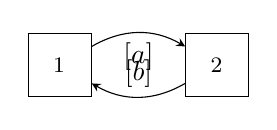
\begin{tikzpicture}[node distance=1.5cm,scale=1]
        \node (square-h) [draw,minimum width=0.8cm,minimum height=0.8cm] {\large $\hh_1$};
        \node (square-k) [draw,minimum width=0.8cm,minimum height=0.8cm, right of = square-h, xshift=5mm] {\large $\hh_2$};
       % 
      \path
      (square-h) edge[-stealth,bend left] node[below] {$\msg[a]$} (square-k)
      (square-k) edge[-stealth,bend left] node[above] {$\msg[b]$} (square-h)
      ;
 \end{tikzpicture}
 }
 %
 \hspace{8mm}
 %
\begin{array}{l}
\text{$\cs_2$}\\[12mm]
\end{array}
 \dbox{
 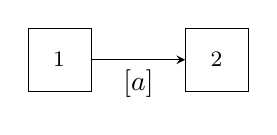
\begin{tikzpicture}[node distance=1.5cm,scale=1]
        \node (square-h) [draw,minimum width=0.8cm,minimum height=0.8cm] {\large $\hh_1$};
        \node (square-k) [draw,minimum width=0.8cm,minimum height=0.8cm, right of = square-h, xshift=5mm] {\large $\hh_2$};
       % 
      \path
      (square-h) edge[-stealth] node[below] {$\msg[a]$} (square-k)
      ;
 \end{tikzpicture} 
        }
 %
 \hspace{8mm}
 %
\begin{array}{l}
\text{$\cs_3$}\\[12mm]
\end{array}
 \dbox{
 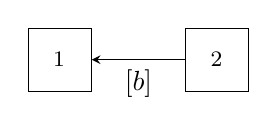
\begin{tikzpicture}[node distance=1.5cm,scale=1]
        \node (square-h) [draw,minimum width=0.8cm,minimum height=0.8cm] {\large $\hh_1$};
        \node (square-k) [draw,minimum width=0.8cm,minimum height=0.8cm, right of = square-h, xshift=5mm] {\large $\hh_2$};
       % 
      \path
      (square-k) edge[-stealth] node[below] {$\msg[b]$} (square-h)
      ;
 \end{tikzpicture} 
        }
 \end{equation}
%  $
% \caption{\label{fig:pcm} Three connection models for composing the systems in \cref{fig:twoipnterfaces}}
% }
%\end{figure}

Notice that the connection models depends only on the choosen interface interactions.
This holds however only for the binary case.
Not for the multicomposition (see below).

The following partial gateways can be obtained out of the interface participants and the connection
models.
\begin{equation}
\hspace{-8mm}
\begin{tikzpicture}[node distance=1.5cm,scale=1]
        \node (square-v)  [draw,minimum width=0.8cm,minimum height=0.8cm] {\large $\hh_3$};
        \node [state] (v-b) [left of = square-v, draw=none] {};
        \node [state] (v-a) [below of = square-v, draw=none] {};
        \draw [-stealth] (v-a) --  node {$\msg[a]$} (square-v);
        \draw [-stealth] (square-v) --  node {$\msg[b]$} (v-b);
        \node (square-w)  [draw,minimum width=0.8cm,minimum height=0.8cm, right of = square-v] {\large $\hh_4$};
        \node [state] (w-c) [right of = square-w, draw=none] {};
        \node [state] (w-a) [below of = square-w, draw=none] {};
        \node [state] (w-b) [above right of = square-w, draw=none] {};
        \draw [-stealth] (w-c) --  node {$\msg[c]$} (square-w);
        \draw [-stealth] (square-w) --  node {$\msg[a]$} (w-a);
        \draw [stealth-] (square-w) --  node {$\msg[b]$} (w-b);
        %
        \draw [-stealth] (square-w) to[out=-135,in=-45]  node {$\msg[b]$} (square-v);
        %
        \draw (0.4,0)[dotted,thick]  --  (0,-0.4); % carrying a inside v
        \draw (0.4,-0.4)[dotted,thick]  --  (-0.4,0); % carrying b inside v
        %
        \draw (1.5,0.4)[dotted,thick]  --  (1.5,-0.4); % carrying a inside w
        \draw (1.1,-0.4)[dotted,thick]  to[out=30,in=260]  (1.9,0.4); % carrying b inside w
        %
        %
        \draw [-stealth]  (0.4,0) to[out=45,in=90]  node [pos=0.6] {$\msg[a]$} (1.5,0.4 ); % carryng a from v to w  
 \end{tikzpicture}
 \hspace{0mm}
 \begin{tikzpicture}[node distance=1.5cm,scale=1]
        \node (square-v)  [draw,minimum width=0.8cm,minimum height=0.8cm] {\large $\hh_3$};
        \node [state] (v-b) [left of = square-v, draw=none] {};
        \node [state] (v-a) [below of = square-v, draw=none] {};
        \draw [-stealth] (v-a) --  node {$\msg[a]$} (square-v);
        \draw [-stealth] (square-v) --  node {$\msg[b]$} (v-b);
        \node (square-w)  [draw,minimum width=0.8cm,minimum height=0.8cm, right of = square-v] {\large $\hh_4$};
        \node [state] (w-c) [right of = square-w, draw=none] {};
        \node [state] (w-a) [below of = square-w, draw=none] {};
        \node [state] (w-b) [above right of = square-w, draw=none] {};
        \draw [-stealth] (w-c) --  node {$\msg[c]$} (square-w);
        \draw [-stealth] (square-w) --  node {$\msg[a]$} (w-a);
        \draw [stealth-] (square-w) --  node {$\msg[b]$} (w-b);
        %
        \draw [-stealth] (square-w) to[out=-135,in=-45]  node {$\msg[b]$} (square-v);
        %
        %\draw (0.4,0)[dotted,thick]  --  (0,-0.4); % carrying a inside v
        \draw (0.4,-0.4)[dotted,thick]  --  (-0.4,0); % carrying b inside v
        %
        %\draw (1.5,0.4)[dotted,thick]  --  (1.5,-0.4); % carrying a inside w
        \draw (1.1,-0.4)[dotted,thick]  to[out=30,in=260]  (1.9,0.4); % carrying b inside w
        %
        %
       % \draw [-stealth]  (0.4,0) to[out=45,in=90]  node [pos=0.6] {$\msg[a]$} (1.5,0.4 ); % carryng a from v to w  
 \end{tikzpicture}
 \hspace{0mm}
\begin{tikzpicture}[node distance=1.5cm,scale=1]
        \node (square-v)  [draw,minimum width=0.8cm,minimum height=0.8cm] {\large $\hh_3$};
        \node [state] (v-b) [left of = square-v, draw=none] {};
        \node [state] (v-a) [below of = square-v, draw=none] {};
        \draw [-stealth] (v-a) --  node {$\msg[a]$} (square-v);
        \draw [-stealth] (square-v) --  node {$\msg[b]$} (v-b);
        \node (square-w)  [draw,minimum width=0.8cm,minimum height=0.8cm, right of = square-v] {\large $\hh_4$};
        \node [state] (w-c) [right of = square-w, draw=none] {};
        \node [state] (w-a) [below of = square-w, draw=none] {};
        \node [state] (w-b) [above right of = square-w, draw=none] {};
        \draw [-stealth] (w-c) --  node {$\msg[c]$} (square-w);
        \draw [-stealth] (square-w) --  node {$\msg[a]$} (w-a);
        \draw [stealth-] (square-w) --  node {$\msg[b]$} (w-b);
        %
        %\draw [-stealth] (square-w) to[out=-135,in=-45]  node {$\msg[b]$} (square-v);
        %
        \draw (0.4,0)[dotted,thick]  --  (0,-0.4); % carrying a inside v
        %\draw (0.4,-0.4)[dotted,thick]  --  (-0.4,0); % carrying b inside v
        %
        \draw (1.5,0.4)[dotted,thick]  --  (1.5,-0.4); % carrying a inside w
        %
        %
        \draw [-stealth]  (0.4,0) to[out=45,in=90]  node [pos=0.6] {$\msg[a]$} (1.5,0.4 ); % carryng a from v to w  
 \end{tikzpicture}
\end{equation}




This approach to composition easily scales up to general multiple composition. 

Let us consider an example from~\cite{BDGY23} having four systems $S_1$,  $S_2$, $S_3$ and $S_4$.
As shown in (\ref{eq:four-ips}) below, we have selected for each system one participant
as an interface, named respectively $\hh_1$, $\hh_2$, $\hh_3$ and $\hh_4$.
 
%\begin{wrapfigure}{r}{0.45\textwidth}
%\begin{figure}[h]
%    %\vspace{-8mm}
%     \centering{\small
%    $
\begin{equation}
\label{eq:four-ips}
    \begin{array}{@{\hspace{0mm}}c@{\hspace{-2mm}}}
    \begin{array}{c@{\hspace{-2mm}}c}
    \text{\large $S_1$}
    &
 \begin{tikzpicture}[node distance=1.5cm,scale=1]
        \node (square-h) [draw,minimum width=0.8cm,minimum height=0.8cm] {\large $\hh_1$};
        \node [state] (h-a) [above of = square-h, draw=none] {};
        \node [state] (h-c) [left of = square-h, draw=none] {};
        \draw [-stealth] (h-a) --  node {$\msg[a]$} (square-h);
        \draw [-stealth] (square-h) --  node {$\msg[c]$} (h-c);
 \end{tikzpicture}
 \end{array}
 \hspace{4mm}
\begin{array}{c}
 \\
 \\
| \\
| \\
|\\
|\\
\end{array}
 \hspace{4mm}
 \begin{array}{c@{\hspace{-2mm}}c}
\begin{tikzpicture}[node distance=1.5cm,scale=1]
        \node (square-k) [draw,minimum width=0.8cm,minimum height=0.8cm] {\large $\hh_2$};
        \node [state] (k-b) [above of = square-k, draw=none] {};
        \node [state] (k-a) [right of = square-k, draw=none] {};
        \draw [-stealth] (k-b) --  node {$\msg[b]$} (square-k);
        \draw [-stealth] (square-k) --  node {$\msg[a]$} (k-a);
 \end{tikzpicture}
 &
 \text{\large $S_2$} 
 \end{array}
 \\[12mm]
\hspace{3mm}- - - -    \hspace{8mm}- - - - -  \\[-5mm]
\begin{array}{@{\hspace{0mm}}c@{\hspace{0mm}}c}
\\[4mm]
\text{\large $S_3\hspace{-2mm}$} 
&
 \begin{tikzpicture}[node distance=1.5cm,scale=1]
        \node (square-v) [draw,minimum width=0.8cm,minimum height=0.8cm] {\large $\hh_3$};
        \node [state] (v-b) [left of = square-v, draw=none] {};
        \node [state] (v-a) [below of = square-v, draw=none] {};
        \draw [-stealth] (v-a) --  node {$\msg[a]$} (square-v);
        \draw [-stealth] (square-v) --  node {$\msg[b]$} (v-b);
 \end{tikzpicture}
 \end{array}
 \hspace{4mm}
\begin{array}{c}
 \\[-8mm]
| \\
| \\
| \\
|
\end{array}
 \hspace{4mm}
 \begin{array}{c@{\hspace{-2mm}}}
 \\[-6mm]
 \begin{tikzpicture}[node distance=1.5cm,scale=1]
        \node (square-w) [draw,minimum width=0.8cm,minimum height=0.8cm] {\large $\hh_4$};
        \node [state] (w-c) [right of = square-w, draw=none] {};
        \node [state] (w-a) [below of = square-w, draw=none] {};
        \node [state] (w-b) [above right of = square-w, draw=none] {};
        \draw [-stealth] (w-c) --  node {$\msg[c]$} (square-w);
        \draw [-stealth] (square-w) --  node {$\msg[a]$} (w-a);
        \draw [stealth-] (square-w) --  node {$\msg[b]$} (w-b);
 \end{tikzpicture}
 \hspace{-6mm}
 \begin{array}{l}
 \\[6mm]
 \text{\large\ \ $S_4$}
 \end{array} 
 \end{array}
 \\[-4mm]
 \end{array}
 \end{equation}
% $
% }
%\caption{\label{fig:four-ips}
%Four systems with their respective interface participants}
% \end{figure}
% \vspace{-5mm}
% \end{wrapfigure}

We could take into account the following interface actions.

%\begin{figure}[h]
%    %\vspace{-8mm}
%     \centering{\small
%    $
\begin{equation}
\label{eq:four-ips}
    \begin{array}{@{\hspace{0mm}}c@{\hspace{-2mm}}}
    \begin{array}{c@{\hspace{-2mm}}c}
    \text{\large $S_1$}
    &
 \begin{tikzpicture}[node distance=1.5cm,scale=1]
        \node (square-h) [draw,minimum width=0.8cm,minimum height=0.8cm] {\large $\hh_1$};
        \node [state] (h-a) [above of = square-h, draw=none] {};
        \node [state] (h-c) [left of = square-h, draw=none] {};
        \draw [-stealth,line width=0.5mm] (h-a) --  node [right] {$\msg[a]$} (square-h);
        \draw [-stealth] (square-h) --  node {$\msg[c]$} (h-c);
 \end{tikzpicture}
 \end{array}
 \hspace{4mm}
\begin{array}{c}
 \\
 \\
| \\
| \\
|\\
|\\
\end{array}
 \hspace{4mm}
 \begin{array}{c@{\hspace{-2mm}}c}
\begin{tikzpicture}[node distance=1.5cm,scale=1]
        \node (square-k) [draw,minimum width=0.8cm,minimum height=0.8cm] {\large $\hh_2$};
        \node [state] (k-b) [above of = square-k, draw=none] {};
        \node [state] (k-a) [right of = square-k, draw=none] {};
        \draw [-stealth, line width=0.5mm] (k-b) --  node [right] {$\msg[b]$} (square-k);
        \draw [-stealth, line width=0.5mm] (square-k) --  node [below] {$\msg[a]$} (k-a);
 \end{tikzpicture}
 &
 \text{\large $S_2$} 
 \end{array}
 \\[12mm]
\hspace{3mm}- - - -    \hspace{8mm}- - - - -  \\[-5mm]
\begin{array}{@{\hspace{0mm}}c@{\hspace{0mm}}c}
\\[4mm]
\text{\large $S_3\hspace{-2mm}$} 
&
 \begin{tikzpicture}[node distance=1.5cm,scale=1]
        \node (square-v) [draw,minimum width=0.8cm,minimum height=0.8cm] {\large $\hh_3$};
        \node [state] (v-b) [left of = square-v, draw=none] {};
        \node [state] (v-a) [below of = square-v, draw=none] {};
        \draw [-stealth,line width=0.5mm] (v-a) --  node [right]   {$\msg[a]$} (square-v);
        \draw [-stealth,line width=0.5mm] (square-v) --  node [below] {$\msg[b]$} (v-b);
 \end{tikzpicture}
 \end{array}
 \hspace{4mm}
\begin{array}{c}
 \\[-8mm]
| \\
| \\
| \\
|
\end{array}
 \hspace{4mm}
 \begin{array}{c@{\hspace{-2mm}}}
 \\[-6mm]
 \begin{tikzpicture}[node distance=1.5cm,scale=1]
        \node (square-w) [draw,minimum width=0.8cm,minimum height=0.8cm] {\large $\hh_4$};
        \node [state] (w-c) [right of = square-w, draw=none] {};
        \node [state] (w-a) [below of = square-w, draw=none] {};
        \node [state] (w-b) [above right of = square-w, draw=none] {};
        \draw [-stealth] (w-c) --  node {$\msg[c]$} (square-w);
        \draw [-stealth,line width=0.5mm] (square-w) --  node [right] {$\msg[a]$} (w-a);
        \draw [stealth-] (square-w) --  node {$\msg[b]$} (w-b);
 \end{tikzpicture}
 \hspace{-6mm}
 \begin{array}{l}
 \\[6mm]
 \text{\large\ \ $S_4$}
 \end{array} 
 \end{array}
 \\[-4mm]
 \end{array}
 \end{equation}
% $
% }
%\caption{\label{fig:four-ips}
%Four interfaces with particular interface actions.}
% \end{figure}
% \vspace{-5mm}
% \end{wrapfigure}

Unlike the binary case, a connection policy is not uniquely determined the specification
of which are the interface actions in the interface participants.

For what concerns  the choice of interface actions highlighted in (\ref{eq:four-ips}),
 one could decide that message $\msg[a]$ received by $\hh_1$ has 
 to be forwarded
 to $\hh_4$; the $\msg[a]$ received by $\hh_3$
 to $\hh_2$; the $\msg[b]$ received by $\hh_2$ to $\hh_3$.
 Another possible choice 
could be similar to the previous one but for the forwarding
of the messages $\msg[a]$: the one received by $\HH_1$ could be forwarded now to $\hh_2$
whereas the one received by $\hh_3$ could be forwarded to $\hh_4$. 
So, it is possible to have the following two connection models, both coherent
with the interface actions highlighted in (\ref{fig:four-ips}).  
 

%%% CONNECTION MODELS
% \begin{figure}[ht]
%    \centering{
 \begin{equation}
    \raisebox{15mm}{$\cs_\mathrm{A}$}
    \begin{array}{c@{\qquad\qquad\qquad\qquad\qquad}c}
\dbox{
 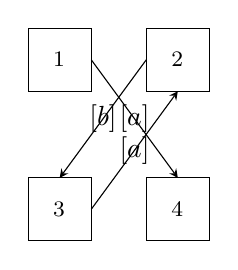
\begin{tikzpicture}[node distance=1.5cm,scale=1]
        \node (square-h) [draw,minimum width=0.8cm,minimum height=0.8cm] {\large $\hh_1$};
        \node (square-k) [draw,minimum width=0.8cm,minimum height=0.8cm, right of = square-h] {\large $\hh_2$};
        \node (square-v)  [draw,minimum width=0.8cm,minimum height=0.8cm, below of = square-h, yshift=-4mm] {\large $\hh_3$};
        \node (square-w)  [draw,minimum width=0.8cm,minimum height=0.8cm, below of = square-k, yshift=-4mm] {\large $\hh_4$};
        %\draw[-stealth]  (square-w) to[out=-135,in=-45]  node {$\msg[b]$} (square-v);
        %
        %
        \draw [-stealth] (0.4,0)  -- node {$\msg[a]$}  (1.5,-1.5 ); % carryng a from h to w    
        % \draw [stealth-] (0,-0.4)  -- node {$\msg[c]$} (1.1,-1.9); % carryng c from w to h 
        \draw [-stealth] (0.4,-1.9)  --  node {$\msg[a]$} (1.5,-0.4 ); % carrying a from v to k
        \draw [stealth-] (0,-1.5)  --  node {$\msg[b]$} (1.1,0); % carrying  b from k to v
 \end{tikzpicture}
 }
&
\dbox{
 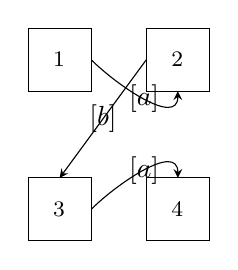
\begin{tikzpicture}[node distance=1.5cm,scale=1]
        \node (square-h) [draw,minimum width=0.8cm,minimum height=0.8cm] {\large $\HH_1$};
        \node (square-k) [draw,minimum width=0.8cm,minimum height=0.8cm, right of = square-h] {{\large $\hh_2$}};
        \node (square-v)  [draw,minimum width=0.8cm,minimum height=0.8cm, below of = square-h, yshift=-4mm] {{\large $\hh_3$}};
        \node (square-w)  [draw,minimum width=0.8cm,minimum height=0.8cm, below of = square-k, yshift=-4mm] {{\large $\hh_4$}};
        %
        %\draw [-stealth] (square-w) to[out=-135,in=-45]  node {$\msg[b]$} (square-v);
        %
        %
        \draw [-stealth] (0.4,-1.9) to[out=45,in=90] node {$\msg[a]$} (1.5,-1.5 ); % carryng a from v to w    
         %\draw [stealth-] (0,-0.4)  -- node {$\msg[c]$} (1.1,-1.9) ; % carryng c from w to h 
        \draw [-stealth]  (0.4,0)  to[out=-45,in=-90]  node {$\msg[a]$} (1.5,-0.4 ); % carrying a from h to k
        %\draw [-stealth]  (square-v)  to[out=45,in=-90]  node {$\msg[a]$} (square-k); % carrying a from h to k
        \draw [stealth-] (0,-1.5)  --  node {$\msg[b]$} (1.1,0); % carrying  b from k to v
 \end{tikzpicture}
 }
 \raisebox{14.5mm}{$\,\,\,\,\cs_\mathrm{B}$}
 \end{array}
  \end{equation}
% $
% }
% \caption{\label{fig:choicesAB} Two connection models for multicomposition.}\label{fig:twocm}
% \end{figure}
 
 \noindent
  Similarly to the binary case, the PaI multicomposition via partial gateways of the four
 systems consists in fact in replacing the participants  $\hh_1$, $\hh_2$, $\hh_3$ and $\hh_4$, chosen  as
interfaces, by gateways whose task stays the same for what concerns the non interface-actions,
whereas messages of interfaces actions are simply forwarded.
 The  architecture  of the resulting composed systems, according to the connection models is
represented  by the diagrams  in (\ref{eq:multiconnection}),  where the names $\hh_1, \hh_2, \hh_3$
and $\hh_4$ are now partial gateways.
%\begin{figure}[h]%{c}{0.6\textwidth}
%\vspace{-4mm}
%    \centering{
\vspace{-4mm} 
\begin{equation}
 \label{eq:multiconnection}
    \begin{array}{c@{\quad\qquad}c}
 \begin{tikzpicture}[node distance=1.5cm,scale=1]
        \node (square-h) [draw,minimum width=0.8cm,minimum height=0.8cm] {\large $\hh_1$};
        \node [state] (h-a) [above of = square-h, draw=none] {};
        \node [state] (h-c) [left of = square-h, draw=none] {};
        \draw [-stealth] (h-a) --  node {$\msg[a]$} (square-h);
        \draw [-stealth] (square-h) --  node {$\msg[c]$} (h-c);
        \node (square-k) [draw,minimum width=0.8cm,minimum height=0.8cm, right of = square-h] {\large $\hh_2$};
        \node [state] (k-b) [above of = square-k, draw=none] {};
        \node [state] (k-a) [right of = square-k, draw=none] {};
        \draw [-stealth] (k-b) --  node {$\msg[b]$} (square-k);
        \draw [-stealth] (square-k) --  node {$\msg[a]$} (k-a);
        \node (square-v)  [draw,minimum width=0.8cm,minimum height=0.8cm, below of = square-h, yshift=-4mm] {\large $\hh_3$};
        \node [state] (v-b) [left of = square-v, draw=none] {};
        \node [state] (v-a) [below of = square-v, draw=none] {};
        \draw [-stealth] (v-a) --  node {$\msg[a]$} (square-v);
        \draw [-stealth] (square-v) --  node {$\msg[b]$} (v-b);
        \node (square-w)  [draw,minimum width=0.8cm,minimum height=0.8cm, below of = square-k, yshift=-4mm] {\large $\hh_4$};
        \node [state] (w-c) [right of = square-w, draw=none] {};
        \node [state] (w-a) [below of = square-w, draw=none] {};
        \node [state] (w-b) [above right of = square-w, draw=none] {};
        \draw [-stealth] (w-c) --  node {$\msg[c]$} (square-w);
        \draw [-stealth] (square-w) --  node {$\msg[a]$} (w-a);
        \draw [stealth-] (square-w) --  node {$\msg[b]$} (w-b);
        %
      %  \draw (square-h)  to[out=-90,in=90]   node {} (square-w);
       % \draw (square-k) to[out=-90,in=90]  node {} (square-v);
      %  \draw (square-h) to[out=0,in=180]  node {} (square-w);
      %  \draw [-stealth] (square-w) to[out=-135,in=-45]  node {$\msg[b]$} (square-v);
      %  \draw (square-k) to[out=-135,in=45]  node {} (square-v);
        %
        \draw (0,0.4)[dotted,thick]  --  (0.4,0); % carrying a inside h  
        %\draw (-0.4,0)[dotted,thick]  --  (0,-0.4); % carrying c inside h
        %
        \draw (1.5,0.4)[dotted,thick]  --  (1.1,0); % carrying b inside k
        \draw (1.5,-0.4)[dotted,thick]  --  (1.9,0); % carrying a inside k
        %
        \draw (0.4,-1.9)[dotted,thick]  --  (0,-2.3); % carrying a inside v
        \draw (0,-1.5)[dotted,thick]  --  (-0.4,-1.9); % carrying k's b inside v
        %\draw (0.4,-2.3)[dotted,thick]  --  (-0.4,-1.9); % carrying b inside v
        %
        \draw (1.5,-1.5)[dotted,thick]  --  (1.5,-2.3); % carrying a inside w
        %\draw (1.1,-1.9)[dotted,thick]  --  (1.9,-1.9); % carrying c inside w
        %\draw (1.1,-2.3)[dotted,thick]  to[out=30,in=260]  (1.9,-1.5); % carrying b inside w
        %
        %
        \draw[-stealth]   (0.4,0)  -- node  {$\msg[a]$}   (1.5,-1.5 ); % carryng a from h to w    
         %\draw  [stealth-]  (0,-0.4)  --  node  {$\msg[c]$}  (1.1,-1.9); % carryng c from w to h 
        \draw [-stealth]  (0.4,-1.9)  --   node  {$\msg[a]$} (1.5,-0.4 ); % carrying a from v to k
        \draw [stealth-]  (0,-1.5)  --  node {$\msg[b]$} (1.1,0); % carrying  b from k to v
 \end{tikzpicture}
& 
\begin{tikzpicture}[node distance=1.5cm,scale=1]
        \node (square-h) [draw,minimum width=0.8cm,minimum height=0.8cm] {\large $\HH$};
        \node [state] (h-a) [above of = square-h, draw=none] {};
        \node [state] (h-c) [left of = square-h, draw=none] {};
        \draw [-stealth] (h-a) --  node {$\msg[a]$} (square-h);
        \draw [-stealth] (square-h) --  node {$\msg[c]$} (h-c);
        \node (square-k) [draw,minimum width=0.8cm,minimum height=0.8cm, right of = square-h] {\large $\KK$};
        \node [state] (k-b) [above of = square-k, draw=none] {};
        \node [state] (k-a) [right of = square-k, draw=none] {};
        \draw [-stealth] (k-b) --  node {$\msg[b]$} (square-k);
        \draw [-stealth] (square-k) --  node {$\msg[a]$} (k-a);
        \node (square-v)  [draw,minimum width=0.8cm,minimum height=0.8cm, below of = square-h, yshift=-4mm] {\large $\hh_3$};
        \node [state] (v-b) [left of = square-v, draw=none] {};
        \node [state] (v-a) [below of = square-v, draw=none] {};
        \draw [-stealth] (v-a) --  node {$\msg[a]$} (square-v);
        \draw [-stealth] (square-v) --  node {$\msg[b]$} (v-b);
        \node (square-w)  [draw,minimum width=0.8cm,minimum height=0.8cm, below of = square-k, yshift=-4mm] {\large $\hh_4$};
        \node [state] (w-c) [right of = square-w, draw=none] {};
        \node [state] (w-a) [below of = square-w, draw=none] {};
        \node [state] (w-b) [above right of = square-w, draw=none] {};
        \draw [-stealth] (w-c) --  node {$\msg[c]$} (square-w);
        \draw [-stealth] (square-w) --  node {$\msg[a]$} (w-a);
        \draw [stealth-] (square-w) --  node {$\msg[b]$} (w-b);
        %
        %\draw [-stealth] (square-w) to[out=-135,in=-45]  node {$\msg[b]$} (square-v);
        %
        \draw (0,0.4)[dotted,thick]  --  (0.4,0); % carrying a inside h  
        %\draw (-0.4,0)[dotted,thick]  --  (0,-0.4); % carrying c inside h
        %
        \draw (1.5,0.4)[dotted,thick]  --  (1.1,0); % carrying b inside k
        \draw (1.5,-0.4)[dotted,thick]  --  (1.9,0); % carrying a inside k
        %
        \draw (0.4,-1.9)[dotted,thick]  --  (0,-2.3); % carrying a inside v
        \draw (0,-1.5)[dotted,thick]  --  (-0.4,-1.9); % carrying k's b inside v
        %\draw (0.4,-2.3)[dotted,thick]  --  (-0.4,-1.9); % carrying b inside v
        %
        \draw (1.5,-1.5)[dotted,thick]  --  (1.5,-2.3); % carrying a inside w
        %\draw (1.1,-1.9)[dotted,thick]  --  (1.9,-1.9); % carrying c inside w
        %\draw (1.1,-2.3)[dotted,thick]  to[out=30,in=260]  (1.9,-1.5); % carrying b inside w
        %
        %
        \draw [-stealth]  (0.4,-1.9) to[out=45,in=90]  node [pos=0.6] {$\msg[a]$} (1.5,-1.5 ); % carryng a from v to w    
         %\draw [stealth-]  (0,-0.4)  --  node  {$\msg[c]$} (1.1,-1.9); % carryng c from w to h 
        \draw [-stealth]  (0.4,0)  to[out=-45,in=-90]  node [pos=0.6]  {$\msg[a]$} (1.5,-0.4 ); % carrying a from h to k
        \draw [stealth-]  (0,-1.5)  -- node  {$\msg[b]$}  (1.1,0); % carrying  b from k to v
 \end{tikzpicture}\\[-4mm]
 \text{\small (Using $\cs_\mathrm{A}$)}
 &
 \text{\small (Using $\cs_\mathrm{B}$)}
 \end{array}
  \end{equation}
 
%  }
%  \vspace{-1mm}
%  \caption{Static description of two PaI multicompositions via partial gateways}
%  \label{fig:multiconnection}
% \end{figure}

One of the main results of the paper is that a number of comminication properties
are preserved by PaI multicomposition via partial gateways in case the very same
properties are enjoied by the connection policy used for the composition.
Such a result is actually obtained as a corollary of a preservation result for 
a restricted form of binary PaI composition that we dub partial-fusion PaI composition.
All forms of PaI composition for asynchronous CFSM can be obtained by a number
of binary partial-fusion PaI composition, which can hence be considered as the 
basis of the PaI approach.

\paragraph{Partial Fusion PaI Composition}

This particular form of PaI composition is binary.
To get an intuitive idea of that, let us consider the following simple example, where
both $S_1$ and $S_2$ possess a participant named $\hh$ that we choose as
their respective interface participant.

\begin{equation}
\label{eq:exps}
\raisebox{2mm}{\text{\large $S_1$}\,\,}
%    \dbox{
\hspace{10mm} \begin{tikzpicture}[node distance=1.5cm,scale=1]
        \node (square-h) [draw,minimum width=0.8cm,minimum height=0.8cm] {\large $\hh$};
        \node [state] (h-a) [above of = square-h, draw=none] {};
        \node [state] (h-c) [left of = square-h, draw=none, xshift=-2mm] {};
        \draw [-stealth] (h-a) --  node {$\msg[a]$} (square-h);
        \draw [stealth-] (h-c) --  node {$\msg[b]$} (square-h);
 \end{tikzpicture}
%            }
\hspace{2mm}
 \begin{array}{c}
 \\[8mm]
| \\
| \\
|\\
|\\
\end{array}
\hspace{4mm}
%     \dbox{
 \begin{tikzpicture}[node distance=1.5cm,scale=1]
        \node (square-k) [draw,minimum width=0.8cm,minimum height=0.8cm] {\large $\hh$};
        \node [state] (k-b) [above of = square-k, draw=none] {};
        \node [state] (k-a) [right of = square-k, draw=none] {};
        %\draw [stealth-] (k-b) --  node[right] {$\msg[inf]$} (square-k);
        \draw [-stealth] (square-k) --  node {$\msg[a]$} (k-a);
       % \draw  [-stealth] (0.4,-0.2)   --  node [below] {$\msg[par]$} (1.2,-0.2);
 \end{tikzpicture} \hspace{18mm}
 %            }
 \raisebox{0mm}{\text{\large $\,\,S_2$}}
 \end{equation}
 
The composition method requires that some interaction actions are choosen in only one
of the two interface participants.  

\begin{equation}
\label{eq:expsia}
\begin{array}{c}
\\[-18mm]
\raisebox{2mm}{\text{\large $S_1$}\,\,}
%    \dbox{
\hspace{10mm} \begin{tikzpicture}[node distance=1.5cm,scale=1]
        \node (square-h) [draw,minimum width=0.8cm,minimum height=0.8cm] {\large $\hh$};
        \node [state] (h-a) [above of = square-h, draw=none] {};
        \node [state] (h-c) [left of = square-h, draw=none, xshift=-2mm] {};
        \draw [-stealth,line width=0.5mm] (h-a) --  node[right] {$\msg[a]$} (square-h);
        \draw [stealth-] (h-c) --  node {$\msg[b]$} (square-h);
 \end{tikzpicture}
%            }
\hspace{2mm}
 \begin{array}{c}
 \\[8mm]
| \\
| \\
|\\
|\\
\end{array}
\hspace{4mm}
%     \dbox{
 \begin{tikzpicture}[node distance=1.5cm,scale=1]
        \node (square-k) [draw,minimum width=0.8cm,minimum height=0.8cm] {\large $\hh$};
        \node [state] (k-b) [above of = square-k, draw=none] {};
        \node [state] (k-a) [right of = square-k, draw=none] {};
        %\draw [stealth-] (k-b) --  node[right] {$\msg[inf]$} (square-k);
        \draw [-stealth] (square-k) --  node {$\msg[a]$} (k-a);
       % \draw  [-stealth] (0.4,-0.2)   --  node [below] {$\msg[par]$} (1.2,-0.2);
 \end{tikzpicture} \hspace{18mm}
 %            }
 \raisebox{0mm}{\text{\large $\,\,S_2$}}
 \end{array}
 \end{equation}

We ``restrict'' now the behaviour of  $\hh$ in $S_1$ (the interface participant with interface actions)
to its interface actions only.
\begin{equation}
\begin{array}{c}
\\[-18mm]
\begin{tikzpicture}[node distance=1.5cm,scale=1]
        \node (square-h) [draw,minimum width=0.8cm,minimum height=0.8cm] {\large $\hh'$};
        \node [state] (h-a) [above of = square-h, draw=none] {};
        \node [state] (h-c) [left of = square-h, draw=none, xshift=-2mm] {};
        \draw [-stealth] (h-a) --  node {$\msg[a]$} (square-h);
 \end{tikzpicture}
  \end{array}
\end{equation}

The composition can be carried on now, since $\hh'$ above and $\hh$ of $S_2$ in (\ref{eq:expsia}) 
are dual (one has an input where the other has an output end vice versa).
 Such a duality property enables to (partially) fuse together the $\hh$ in $S_1$ with the
 $\hh$ in $S_2$ so obtaining a composed system.
 The fusion makes $\hh$ a single and (partially) forwarding gateway: the messages pertaining to
 interface actions are forwarded, whereas such a partial gateways keeps on behaving as the $\hh$ of $S_1$ for what concerns the non interface-actions.

\begin{equation}
\label{fig:bincomp}
\begin{array}{l}
\text{\large $S_1$}\!\stackrel{\hh}{ \mathtt{fuse}}\text{\large $S_2$}\\[12mm]
\end{array}
\hspace{12mm}
% \dbox{ \hspace{28mm}
 \begin{tikzpicture}[node distance=1.5cm,scale=1]
        \node (square-h) [draw,minimum width=0.8cm,minimum height=0.8cm] {\large $\hh$};
         \node[draw=none,fill=none] (h-a) [above = 6mm  of square-h]{};
         \node[draw=none,fill=none] (a-h) [left = 6mm  of square-h]{};
        \draw [-stealth] (h-a) --  node [right] {$\msg[a]$} (square-h);
        \draw [-stealth] (square-h) --  node {$\msg[b]$} (a-h);
         %
        \draw (0,0.4)[dotted,thick]  --  (0.4,0); 
 \end{tikzpicture}
 \hspace{22mm}
%       }
\end{equation}

\medskip

We prove that fusion-composition preserve a number of communication properties.
Besides, it is possible to show that PaI composition by partial gateways (and hence 
PaI composition by gateways in general) preserve such properties since any 
PaI composition (binary, with multiple systems, orchestrated) simply reduces
to a number of fusion compositions.
We show that with an example for the binary case for the sake of simplicity.
Let us consider the systems $S_1$ and $S_2$ as in (\ref{eq:twointerfaces})
We hence consider the following identification of interface actions.
\begin{equation}
\label{eq:simpleexia}
\begin{array}{c}
\\[-18mm]
\raisebox{4mm}{\text{\large $S_1$}\,\,}
%    \dbox{
\hspace{10mm} \begin{tikzpicture}[node distance=1.5cm,scale=1]
        \node (square-h) [draw,minimum width=0.8cm,minimum height=0.8cm] {\large $\hh_1$};
        \node [state] (h-a) [above of = square-h, draw=none] {};
        \node [state] (h-c) [left of = square-h, draw=none, xshift=-2mm] {};
        \draw [-stealth,line width=0.5mm] (h-a) --  node[right] {$\msg[sbs]$} (square-h);
        \draw [stealth-] (h-c) --  node[above] {$\msg[inf]$} (square-h);
 \end{tikzpicture}
%            }
\hspace{2mm}
 \begin{array}{c}
 \\[8mm]
| \\
| \\
|\\
|\\
\end{array}
\hspace{4mm}
%     \dbox{
 \begin{tikzpicture}[node distance=1.5cm,scale=1]
        \node (square-k) [draw,minimum width=0.8cm,minimum height=0.8cm] {\large $\hh_2$};
        \node [state] (k-b) [above of = square-k, draw=none] {};
        \node [state] (k-a) [right of = square-k, draw=none] {};
        %\draw [stealth-] (k-b) --  node[right] {$\msg[inf]$} (square-k);
        \draw [-stealth,line width=0.5mm] (square-k) --  node[above] {$\msg[sbs]$} (k-a);
        \draw  [-stealth] (0.4,-0.2)   --  node [below] {$\msg[par]$} (1.2,-0.2);
 \end{tikzpicture} \hspace{18mm}
 %            }
 \raisebox{2mm}{\text{\large $\,\,S_2$}}
 \end{array}
 \end{equation}
 

Since we are considering a binary case, the connection policy is uniquely determined.

%\begin{figure}[h]
%    \centering{\small
%    $
\begin{equation}
\label{fig:pcp}
\begin{array}{l}
\text{$\cs$}\\[12mm]
\end{array}
 \dbox{
 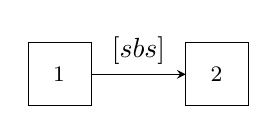
\begin{tikzpicture}[node distance=1.5cm,scale=1]
        \node (square-h) [draw,minimum width=0.8cm,minimum height=0.8cm] {\large $\hh_1$};
        \node (square-k) [draw,minimum width=0.8cm,minimum height=0.8cm, right of = square-h, xshift=5mm] {\large $\hh_2$};
         %
        \draw [-stealth] (0.4,0)  --  node [above] {$\msg[sbs]$} (1.6,0); % carrying sbs from h1 to h2 h2
 \end{tikzpicture}
 }
 \end{equation}
% $
% \caption{\label{fig:pcp} A connection policy for composing the systems in \cref{fig:twoipnterfaces}}
% }
%\end{figure}

Now we consider systems $S_1$ and $\cs$ (recall that also $\cs$ is a system).

% \begin{figure}[h]
%    \centering{\small
%    $
\begin{equation}
\label{fig:twoipnterfaces}
\raisebox{10mm}{\text{\large $S_1$}\,\,}
    \dbox{
\hspace{10mm} \begin{tikzpicture}[node distance=1.5cm,scale=1]
        \node (square-h) [draw,minimum width=0.8cm,minimum height=0.8cm] {\large $\hh_1$};
        \node [state] (h-a) [above of = square-h, draw=none] {};
        \node [state] (h-c) [left of = square-h, draw=none, xshift=-2mm] {};
        \draw [-stealth] (h-a) --  node[right] {$\msg[sbs]$} (square-h);
        \draw [stealth-] (h-c) --  node[above] {$\msg[inf]$} (square-h);
 \end{tikzpicture}
            }
\hspace{12mm}
 \begin{array}{l}
\text{$\cs$}\\[12mm]
\end{array}
 \dbox{
 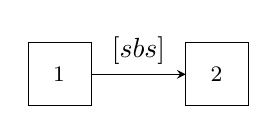
\begin{tikzpicture}[node distance=1.5cm,scale=1]
        \node (square-h) [draw,minimum width=0.8cm,minimum height=0.8cm] {\large $\hh_1$};
        \node (square-k) [draw,minimum width=0.8cm,minimum height=0.8cm, right of = square-h, xshift=5mm] {\large $\hh_2$};
         %
        \draw [-stealth] (0.4,0)  --  node [above] {$\msg[sbs]$} (1.6,0); % carrying sbs from h1 to h2 h2
 \end{tikzpicture}
 }
 \end{equation}
% $\vspace{-2mm}
% \caption{\label{fig:twoipnterfaces} Two interfaces participants belonging to, respectively, systems $S_1$ and $S_2$.}
% }
%\end{figure}

The above system are elegible for fusion composition, which returns the following system.

%\begin{figure}[h]
%    \centering{\small
%    $
\begin{equation}
\label{fig:binpcomp}
\begin{array}{l}
\text{\large $S_1$}\!\stackrel{\hh_1}{ \mathtt{fuse}}\cs\\[22mm]
\end{array}
 \dbox{ \hspace{28mm}
 \begin{tikzpicture}[node distance=1.5cm,scale=1]
        \node (square-h) [draw,minimum width=0.8cm,minimum height=0.8cm] {\large $\hh_1$};
        \draw [-stealth] (h-a) --  node [right] {$\msg[sbs]$} (square-h);
        \node (square-k) [draw,minimum width=0.8cm,minimum height=0.8cm, right of = square-h, xshift=5mm] {\large $\hh_2$};
         \node[draw=none,fill=none] (phantom) [above = 12mm  of square-h]{};
         \node[draw=none,fill=none] (phantom2) [left = 10mm  of square-h]{};
        \draw [stealth-] (phantom2) --  node [above]{$\msg[inf]$} (square-h);
         %
        \draw (0,0.4)[dotted,thick]  --  (0.4,0); % carrying sbs inside h 
        \draw [-stealth] (0.4,0)  -- node [above]{$\msg[sbs]$}  (1.6,0); % carrying sbs from h1 to h2
 \end{tikzpicture}
        }
\end{equation}
% $
% \caption{\label{fig:binpcomp} Pai binary composition via partial gateways}
% }
%\end{figure}

We now consider the following two systems.

%\begin{figure}[h]
%    \centering{\small
%    $
\begin{equation}
\label{fig:binpcomp}
\begin{array}{l}
\text{\large $S_1$}\!\stackrel{\hh_1}{ \mathtt{fuse}}\cs
\\
 \dbox{ \hspace{28mm}
 \begin{tikzpicture}[node distance=1.5cm,scale=1]
        \node (square-h) [draw,minimum width=0.8cm,minimum height=0.8cm] {\large $\hh_1$};
        \draw [-stealth] (h-a) --  node [right] {$\msg[sbs]$} (square-h);
        \node (square-k) [draw,minimum width=0.8cm,minimum height=0.8cm, right of = square-h, xshift=5mm] {\large $\hh_2$};
         \node[draw=none,fill=none] (phantom) [above = 12mm  of square-h]{};
         \node[draw=none,fill=none] (phantom2) [left = 10mm  of square-h]{};
        \draw [stealth-] (phantom2) --  node [above]{$\msg[inf]$} (square-h);
         %
        \draw (0,0.4)[dotted,thick]  --  (0.4,0); % carrying sbs inside h 
        \draw [-stealth] (0.4,0)  -- node [above]{$\msg[sbs]$}  (1.6,0); % carrying sbs from h1 to h2
 \end{tikzpicture}
        }
        \hspace{12mm}
     \dbox{
 \begin{tikzpicture}[node distance=1.5cm,scale=1]
        \node (square-k) [draw,minimum width=0.8cm,minimum height=0.8cm] {\large $\hh_2$};
        \node [state] (k-b) [above of = square-k, draw=none] {};
        \node [state] (k-a) [right of = square-k, draw=none] {};
        %\draw [stealth-] (k-b) --  node[right] {$\msg[inf]$} (square-k);
        \draw [-stealth] (square-k) --  node[above] {$\msg[sbs]$} (k-a);
        \draw  [-stealth] (0.4,-0.2)   --  node [below] {$\msg[par]$} (1.2,-0.2);
 \end{tikzpicture} \hspace{24mm}
             }
 \raisebox{12mm}{\text{\large $\,\,S_2$}}
 \end{array}
 \end{equation}
% $
% \caption{\label{fig:binpcomp} Two systems amenable for fusion composition via $\hh_2$}
% }
%\end{figure}

By applying fusion composition again, we get the following system.

\begin{equation}
\label{fig:bincomp}
\hspace{-22mm}
\begin{array}{l}\big(\text{\large $S_1$}\!\stackrel{\hh_1}{ \mathtt{fuse}}\cs\big)\!\stackrel{\hh_2}{ \mathtt{fuse}}\text{\large $S_2$}\\[22mm]
\end{array}
 \dbox{ \hspace{28mm}
 \begin{tikzpicture}[node distance=1.5cm,scale=1]
        \node (square-h) [draw,minimum width=0.8cm,minimum height=0.8cm] {\large $\hh_1$};
        \draw [-stealth] (h-a) --  node [right] {$\msg[sbs]$} (square-h);
        \node (square-k) [draw,minimum width=0.8cm,minimum height=0.8cm, right of = square-h, xshift=5mm] {\large $\hh_2$};
        \node [state] (k-a) [right of = square-k, draw=none,xshift=2mm] {};
         \node[draw=none,fill=none] (phantom) [above = 12mm  of square-h]{};
         \node[draw=none,fill=none] (phantom2) [left = 10mm  of square-h]{};
        \draw [-stealth] (square-k) --  node [above]{$\msg[sbs]$} (k-a);
        \draw [stealth-] (phantom2) --  node [above]{$\msg[inf]$} (square-h);
         %
        \draw (0,0.4)[dotted,thick]  --  (0.4,0); % carrying sbs inside h 
        \draw [-stealth] (0.4,0)  --  (1.6,0); % carrying sbs from h1 to h2
        \draw  [-stealth] (2.4,-0.2)   --  node [below] {$\msg[par]$} (3.25,-0.2); % carrying par outside h2
        \draw (1.6,0)[dotted,thick]  --  (2.4,0); % carrying sbs inside h2
 \end{tikzpicture}
       }
\end{equation}
 
 We have now that 
 $$
 \big(\text{\large $S_1$}\!\stackrel{\hh_1}{ \mathtt{fuse}}\cs\big)\!\stackrel{\hh_2}{ \mathtt{fuse}}\text{\large $S_2$}\
  \equiv\
   \text{\large $S_1$}\!\stackrel{\hh_1{\leftrightarrow}\hh_2}{ {\mathtt{p\texttt{-}gw}}}\text{\large $S_2$}
 $$
 where $\text{\large $S_1$}\!\stackrel{\hh_1{\leftrightarrow}\hh_2}{ {\mathtt{p\texttt{-}gw}}}\text{\large $S_2$}$ is the system obtained from $S_1$ and $S_2$ by PaI composition via partial gateways using the connection policy $\cs$.

 
 
 




